\chapter{روش تطبیقی مرتبهٔ دوم برای آموزش سریع}
\label{ch:method}

\section{هدف و دامنهٔ تحلیل}
\label{sec:method-overview}

دیدگاه هندسی فصل~\ref{ch:geometry} نشان داد که اندازهٔ بزرگ‌تر گام لزوماً حملهٔ تک‌گامی قوی‌تری تولید نمی‌کند. اگر هزینه در امتداد جهت حمله ابتدا افزایش و سپس کاهش یابد، رسیدن به انتهای بازه می‌تواند یک نمونهٔ هم‌آورد غیرعادی بسازد. روش \sora{} از این مشاهده برای تنظیم دامنهٔ گام استفاده می‌کند: دو شیب موجود در آموزش، اطلاعاتی دربارهٔ تغییر محلی هزینه فراهم می‌کنند و یک کنترل‌کنندهٔ هموارشده، دامنهٔ نمونه‌برداری گام‌های بعدی را تغییر می‌دهد \cite{sora2026}. در این فصل، ابتدا مسئلهٔ دقیق روی یک مدل درجه‌دو حل می‌شود و سپس فاصلهٔ این حل با قاعدهٔ عملی مقاله مشخص می‌گردد.

در سراسر استخراج محلی، برچسب و پارامترهای مدل ثابت‌اند و $\ell(z)=\mathcal{L}(f_\theta(z),y)$ نوشته می‌شود. نقطهٔ آغاز می‌تواند ورودی پاک یا نقطهٔ دارای شروع تصادفی باشد. در این نقطه، $g=\nabla\ell(z)$ و $H=\nabla^2\ell(z)$ را تعریف می‌کنیم. هسین در استدلال حضور دارد، اما در الگوریتم عملی ساخته یا وارون نمی‌شود. این تمایز، معنای استفاده از اطلاعات مرتبهٔ دوم با هزینهٔ کم است: اثر تغییر شیب به‌طور غیرمستقیم در کنترل گام به کار می‌رود، نه اینکه یک روش کامل نیوتنی روی فضای ورودی اجرا شود.

آموزش هم‌آورد استاندارد، بیشینه‌سازی هزینه را در مجموعهٔ تهدید معین دنبال می‌کند \cite{madry2018towards}. با این حال، مولد آموزشی \sora{} دقیقاً حل همین مسئلهٔ مقید با شعاع $\epsilon$ نیست؛ مطابق الگوریتم مقاله، تنها بازهٔ معتبر پیکسل‌ها برش می‌خورد. پیامد این انتخاب در بخش~\ref{sec:method-budget} بیان می‌شود. همچنین همهٔ شکل‌های این فصل بازنشر شواهد و تفسیر مقاله‌اند و نتیجهٔ آزمایش تازه‌ای در این متن محسوب نمی‌شوند.

\section{بیشینه‌سازی اسکالر در جهت علامت شیب}
\label{sec:method-quadratic}

جهت $p=\operatorname{sign}(g)\in\{-1,0,1\}^d$ را پس از محاسبه ثابت می‌گیریم. برای گام اسکالر $a\geq0$، مدل درجه‌دوی هزینه برابر است با
\begin{equation}
q(a)=\ell(z)+a g^{\mathsf T}p+\frac{a^2}{2}p^{\mathsf T}Hp
=\ell(z)+ba+\frac{c}{2}a^2,
\quad b=\|g\|_1,\quad c=p^{\mathsf T}Hp.
\label{eq:method-quadratic}
\end{equation}
اگر $g\ne0$ باشد، $b>0$ است. این جمله همان انگیزهٔ مرتبهٔ اول برای انتخاب جهت علامت است \cite{goodfellow2015explaining}. نقش جملهٔ دوم را علامت $c$ تعیین می‌کند: خمیدگی جهت‌دار، نه مثبت یا منفی بودن همهٔ مقادیر ویژهٔ هسین. یک هسین نامعین نیز می‌تواند در این جهت خاص، خمیدگی منفی یا مثبت داشته باشد.

\begin{لم}[بهینهٔ محدود مدل درجه‌دو]
\label{lem:method-quadratic-optimum}
برای $b>0$ و $A>0$، بیشینه‌ساز $q(a)$ روی بازهٔ $[0,A]$ برابر است با
\begin{equation}
a_{\mathrm{quad}}=
\begin{cases}
\min\{A,-b/c\},&c<0,\\
A,&c\geq0.
\end{cases}
\label{eq:method-quadratic-optimum}
\end{equation}
این نتیجه، بخش دقیق استخراج اندازهٔ گام در تقریب درجه‌دوی مقاله را بیان می‌کند \cite{sora2026}.
\end{لم}

\begin{اثبات}
مشتق‌ها $q'(a)=b+ca$ و $q''(a)=c$ هستند. اگر $c<0$ باشد، تابع اکیداً مقعر است و نقطهٔ ایستای مثبت $-b/c$ بیشینهٔ نامقید آن است. محدود کردن این نقطه به بازهٔ مجاز نتیجهٔ سطر اول را می‌دهد. اگر $c=0$ باشد، تابع با شیب مثبت افزایش می‌یابد و انتهای بازه بهینه است. اگر $c>0$ باشد، برای تمام $a\geq0$ مشتق مثبت است؛ نقطهٔ ایستای منفی یک کمینهٔ خارج از بازه است و باز هم بیشینه در $A$ رخ می‌دهد.
\end{اثبات}

در حالت مقعر، اگر رأس داخل بازه باشد، ادامهٔ حرکت پس از آن هزینه را کاهش می‌دهد. برای مدل \eqref{eq:method-quadratic}، افزایش هزینه نسبت به مبنا در بازهٔ $0<a<-2b/c$ مثبت و پس از آن منفی است. بنابراین عبور از رأس فوراً به معنای غیرعادی شدن نمونه نیست، ولی گام به‌اندازهٔ کافی بلند می‌تواند حتی هزینه را از مقدار اولیه پایین‌تر ببرد. این محاسبه، رابطهٔ گام بیش از حد و نمونهٔ غیرعادی را در یک مدل ساده روشن می‌کند؛ برای سطح واقعی، جمله‌های مرتبهٔ بالاتر و برش ورودی نیز دخالت دارند.

فرض $b>0$ مهم است. اگر $g=0$ باشد، جهت علامت طبق قرارداد صفر می‌شود و مسیر انتخاب‌شده حرکت نمی‌کند. نسبت‌هایی که بر نرم شیب تقسیم می‌شوند نیز تعریف ندارند. در چنین وضعیتی، نظریهٔ حاضر توصیه‌ای برای یافتن جهت تازه از هسین ارائه نمی‌کند. نادیده گرفتن این حالت می‌تواند یک تقسیم عددی پایدارشده را به‌اشتباه به‌عنوان اندازه‌گیری معنادار خمیدگی معرفی کند.

\subsection{بازیابی خمیدگی از یک گام کاوش}
\label{sec:method-probe}

اکنون فرض می‌کنیم هزینه واقعاً درجه‌دو و گام کاوش اسکالرِ معلوم $a_{\mathrm{probe}}>0$ باشد. شیب انتهای همان مسیر برابر است با
\begin{equation}
g_{\mathrm{probe}}=g+a_{\mathrm{probe}}Hp.
\label{eq:method-probe-gradient}
\end{equation}
با ضرب در $p^{\mathsf T}$ و تعریف نسبت
\begin{equation}
r=\frac{p^{\mathsf T}g_{\mathrm{probe}}}{\|g\|_1}
=1+\frac{a_{\mathrm{probe}}c}{b},
\label{eq:method-ratio}
\end{equation}
علامت $r-1$ علامت خمیدگی جهت‌دار را مشخص می‌کند. در حالت $r<1$، رأس دقیق مدل برابر است با
\begin{equation}
a_{\mathrm{vertex}}=-\frac{b}{c}
=\frac{a_{\mathrm{probe}}}{1-r},\qquad
a_{\mathrm{quad}}=\min\left\{A,\frac{a_{\mathrm{probe}}}{1-r}\right\}.
\label{eq:method-exact-probe}
\end{equation}
برای $r\geq1$، پاسخ محدود $A$ است. صورت کسر در رابطهٔ دقیق، اندازهٔ همان گامی است که با آن شیب دوم اندازه‌گیری شده است. مقدار آن یک ثابت دلخواه نیست و حذف این وابستگی، همانی جبری استخراج را تغییر می‌دهد.

نسبت $r$ با \pertalign{} یکسان نیست. \pertalign{} کسینوسی در بازهٔ $[-1,1]$ است، ولی $r$ علاوه بر جهت، اندازهٔ شیب دوم را نیز در خود دارد و ممکن است از این بازه خارج شود. حتی دو شیب کاملاً هم‌راستا می‌توانند نسبت بزرگی یا کوچکی بسازند. پس الگوریتم برای کنترل گام، فقط کسینوس فصل قبل را در فرمول قرار نمی‌دهد. تشخیص این تفاوت برای تفسیر نمودارهای پایش و اجرای درست قاعده ضروری است.

برای مقایسه، اگر جهت ثابت $v=g$ انتخاب شود، جملهٔ خطی $\|g\|_2^2$ و خمیدگی $g^{\mathsf T}Hg$ خواهد بود. در آن حالت، نسبت متناظر را می‌توان به صورت
\begin{equation}
r_g=\frac{g^{\mathsf T}g_{\mathrm{probe}}}{\|g\|_2^2}
=\frac{\|g_{\mathrm{probe}}\|_2}{\|g\|_2}
\cos(g,g_{\mathrm{probe}})
\label{eq:method-gradient-ratio}
\end{equation}
نوشت. این رابطه نشان می‌دهد که حتی در جهت خود شیب نیز کسینوس به‌تنهایی برای تعیین اندازهٔ بهینه کافی نیست. صورت گام کاوش باید حفظ شود و کاربرد اندازهٔ گام استخراج‌شده به همان مقیاس‌بندی جهت وابسته است. جهت $g$ و جهت علامت آن اندازه و هندسهٔ یکسانی ندارند.

\section{از همانی دقیق تا کنترل‌کنندهٔ عملی}
\label{sec:method-practical}

مقاله برای پایداری و استفاده از اطلاعات دسته‌های گذشته، صورت کسر را با ثابت $\alpha_0$ جایگزین می‌کند و قاعدهٔ عملی زیر را به کار می‌گیرد \cite{sora2026}:
\begin{equation}
F(u)=
\begin{cases}
\min\left\{\alpha_{\max},\dfrac{\alpha_0}{1-u}\right\},&u<1,\\
\alpha_{\max},&u\geq1.
\end{cases}
\label{eq:method-controller}
\end{equation}
در این رابطه، $u$ آمارهٔ هموارشدهٔ نسبت است. $\alpha_0$ یک پارامتر تنظیمی با مقیاس اندازهٔ گام و $\alpha_{\max}$ سقف دامنهٔ حمله است. در تنظیم عمومی گزارش‌شدهٔ مقاله، $\alpha_0=0.02$، $\beta=0.05$ و $\alpha_{\max}=2\epsilon$ انتخاب شده‌اند. این اعداد متعلق به روش منتشرشده‌اند و از حل ریاضی مسئلهٔ درجه‌دو به‌طور یکتا نتیجه نمی‌شوند.

برای $u$ نزدیک یک، قاعده به سقف می‌رسد؛ با کاهش کافی $u$، دامنه کوچک می‌شود. این رفتار با پرهیز از عبور از قلهٔ محلی سازگار است. با وجود این، جایگزینی $a_{\mathrm{probe}}$ با $\alpha_0$ به‌طور عمومی بهینگی دقیق رابطهٔ \eqref{eq:method-exact-probe} را حفظ نمی‌کند. کوچک بودن ثابت نیز به‌تنهایی چنین تضمینی نمی‌دهد. تعبیر درست، یک کنترل‌کنندهٔ الهام‌گرفته از مدل درجه‌دو است که پایداری آن با میانگین‌گیری، سقف دامنه و تصادفی‌سازی تقویت می‌شود.

برای نمونهٔ صرفاً تحلیلی $q(a)=q(0)+2a-a^2$، رأس در $a=1$ قرار دارد. اگر گام کاوش $1/4$ باشد، نسبت $r=3/4$ و فرمول دقیق $a_{\mathrm{probe}}/(1-r)=1$ است. استفاده از صورت ثابت $0.02$ در همان نسبت، مقدار $0.08$ را پیش از اعمال سقف می‌دهد. این مثال یک آزمایش روی دادگان نیست؛ تنها نشان می‌دهد که ثابت‌کردن صورت، نتیجهٔ جبری مسئلهٔ اصلی را به قاعده‌ای متفاوت تبدیل می‌کند.

% Source: sora2026 paper Figure 4; already in paper; reproduced conceptual recovery diagram, not a guarantee of recovery for arbitrary models.
\begin{figure}[tbp]
\centering
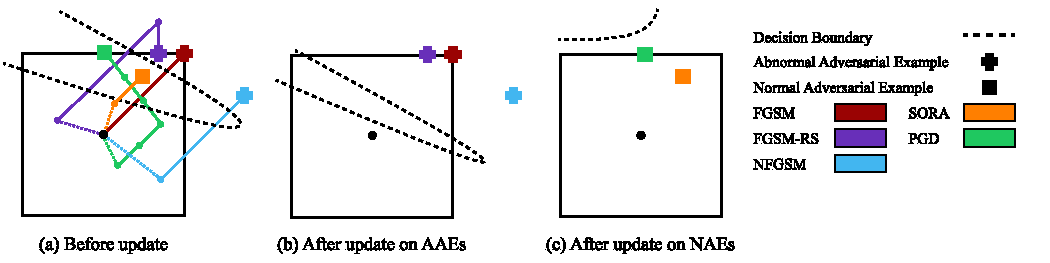
\includegraphics[width=\textwidth]{images/paper_recovery.pdf}
\caption[تفسیر هندسی اصلاح اندازه گام و نمونه‌های غیرعادی]{تفسیر هندسی اصلاح اندازهٔ گام: آموزش روی نمونه‌های غیرعادی ممکن است پیچش مرز تصمیم را تشدید کند، در حالی که دسترسی به نقاط پرهزینه می‌تواند مسیر بازیابی را فراهم سازد. این نمایش سازوکار پیشنهادی را توضیح می‌دهد و تضمین بازیابی پس از هر فروپاشی نیست. بازنشر از شکل ۴ مقالهٔ \sora{} \cite{sora2026}.}
\label{fig:method-recovery}
\end{figure}

\subsection{دامنه‌های تصادفی مؤلفه‌ای}
\label{sec:method-random}

در پیاده‌سازی مفهومی روش، سقف اسکالر $A_i$ برای دستهٔ $i$ تعیین می‌شود، ولی بردار دامنه برای هر نمونه و هر مؤلفه جداگانه نمونه‌برداری می‌شود:
\begin{equation}
a_{i,j}\sim\mathcal{U}(0,A_i),\qquad
\delta_i=a_i\odot p_i,\qquad p_i=\operatorname{sign}(g_i).
\label{eq:method-elementwise}
\end{equation}
شاخص $j$ مؤلفه‌های ورودی، شامل مکان و کانال تصویر، را می‌پیماید و $\odot$ ضرب مؤلفه‌ای است. این انتخاب با نمونه‌برداری یک عدد مشترک برای کل تصویر یا یک عدد مشترک برای هر کانال تفاوت دارد. حتی با علامت ثابت، اندازه‌های نامساوی مؤلفه‌ها جهت هندسی آشفتگی را تغییر می‌دهند. هدف، افزایش تنوع نقاط دیده‌شده و کاهش تمرکز روی یک پوستهٔ ثابت از اندازه‌هاست.

این تصادفی‌سازی نیز فاصله‌ای مشخص با قضیهٔ اسکالر دارد. در مدل درجه‌دو و بدون برش، اگر $D=\operatorname{diag}(a_i)$ باشد، شیب دوم برابر $g+HDp$ است. در نتیجه نسبت مشاهده‌شده شامل $p^{\mathsf T}HDp$ می‌شود، نه لزوماً $a_{\mathrm{probe}}p^{\mathsf T}Hp$. تنها وقتی همهٔ دامنه‌ها برابر باشند، رابطهٔ دقیق کاوش اسکالر مستقیماً بازمی‌گردد. پس $A_i$ سقف یک توزیع است و نباید آن را اندازهٔ واقعی یک گام بهینه برای هر ورودی نامید. با برش پیکسل‌ها، جابه‌جایی واقعی باز هم تغییر می‌کند.

\section{میانگین نمایی و ترتیب زمانی الگوریتم}
\label{sec:method-lag}

در شبه‌کد دسته‌ای این فصل، قرارداد تجمیع برای $B$ نمونه، محاسبهٔ جداگانهٔ نسبت هر نمونه و سپس میانگین‌گیری است:
\begin{equation}
\bar r_i=\frac{1}{B}\sum_{n=1}^{B}
\frac{p_{i,n}^{\mathsf T}g'_{i,n}}{\|g_{i,n}\|_1}.
\label{eq:method-batch-ratio}
\end{equation}
این نگارش، تعمیم صریح نسبت نمونه‌ای به دسته است؛ الگوریتم چاپ‌شده جزئیات این تجمیع را مشخص نمی‌کند. نسبت مجموع صورت‌ها به مجموع مخرج‌ها، به نمونه‌های دارای شیب بزرگ‌تر وزن بیشتری می‌دهد و لزوماً همان آماره نیست. هر قرارداد تجمیع باید هنگام بازتولید روش روشن باشد. برای مخرج صفر نیز باید سیاست عددی مشخصی داشت؛ رابطهٔ نظری تنها برای مخرج مثبت تعریف شده است.

میانگین نمایی با قرارداد مقاله به صورت
\begin{equation}
u_i=(1-\beta)u_{i-1}+\beta\bar r_i,\qquad u_0=0.99
\label{eq:method-ema}
\end{equation}
به‌روزرسانی می‌شود. بنابراین $\beta$ وزن مشاهدهٔ جدید است. برای $\beta=0.05$، کاهش وزن اطلاعات قدیمی در مقیاس چند ده دسته رخ می‌دهد؛ این هموارسازی نویز را کاهش می‌دهد، اما پاسخ به تغییر ناگهانی را کند می‌کند. آمارهٔ مشترک، وضعیت کلی آموزش را خلاصه می‌کند و تضمین نمی‌کند که هر نمونه یا هر زیرگروه دادگان دامنهٔ مناسبی دریافت کند.

ترتیب خطوط ۱۱ و ۱۲ الگوریتم ۱ مقاله نکته‌ای تعیین‌کننده دارد. ابتدا سقف گام دستهٔ بعد با میانگین پیشین محاسبه می‌شود و سپس مشاهدهٔ دستهٔ جاری وارد میانگین می‌گردد. اگر $A_i$ سقف استفاده‌شده در دستهٔ جاری باشد، ترتیب دقیق چنین است:
\begin{equation}
A_{i+1}=F(u_{i-1}),\qquad
u_i=(1-\beta)u_{i-1}+\beta\bar r_i.
\label{eq:method-extra-lag}
\end{equation}
پس مشاهدهٔ دستهٔ $i$ هنوز بر $A_{i+1}$ اثر ندارد و نخست می‌تواند در $A_{i+2}$ ظاهر شود. این یک تأخیر اضافی نسبت به قاعدهٔ «ابتدا میانگین جدید، سپس گام بعد» است. علاوه بر این تأخیر صریح، خود میانگین نمایی حافظهٔ زمانی دارد و شیب‌ها نیز با پارامترهای پیش از به‌روزرسانی جاری اندازه‌گیری شده‌اند.

شبه‌کد~\ref{alg:method-sora} این ترتیب را حفظ می‌کند. برای کامل بودن آغاز اجرا، $A_1=F(u_0)$ در نظر گرفته شده است؛ الگوریتم چاپ‌شده برای نخستین استفاده از سقف، مقداردهی جداگانهٔ روشنی نمایش نمی‌دهد. این قرارداد آغازین، تکمیل اجرایی شبه‌کد است و نباید با یک نتیجهٔ نظری مقاله اشتباه شود. در صورت استفاده از سقف آغازین دیگری، همان مقدار باید در گزارش پیاده‌سازی ثبت شود.

% Source: sora2026 paper Algorithm 1; already in paper; Persian restatement preserving lines 11-before-12, with explicit first-cap initialization and batch reduction.
\begin{algorithm}[tbp]
\caption{بازنویسی \sora{} با حفظ ترتیب زمانی الگوریتم مقاله \cite{sora2026}}
\label{alg:method-sora}
\textbf{ورودی:} مدل $f_\theta$، دسته‌های آموزش، $\epsilon$، $\alpha_0$، $\alpha_{\max}$ و $\beta$.
\begin{enumerate}
\setlength{\itemsep}{0pt}
\item مقداردهی $u_0\gets0.99$، $A_1\gets F(u_0)$ و $i\gets1$.
\item برای هر دستهٔ $(x_i,y_i)$، مراحل ۳ تا ۱۳ را اجرا کنید.
\item برای هر نمونه، $\eta_i\sim\mathcal{U}([-\epsilon,\epsilon]^d)$ و $z_i\gets x_i+\eta_i$.
\item محاسبه $g_i\gets\nabla_{z_i}\mathcal{L}(f_\theta(z_i),y_i)$ و $p_i\gets\operatorname{sign}(g_i)$.
\item جداسازی $p_i$ از گراف ساخت حمله.
\item نمونه‌برداری مستقل $a_{i,j}\sim\mathcal{U}(0,A_i)$ برای مؤلفه‌ها.
\item ساخت $\widetilde x_i\gets\Pi_{[0,1]^d}(x_i+\eta_i+a_i\odot p_i)$.
\item دریافت $(g'_i,g_{\theta,i})\gets\nabla_{(\widetilde x_i,\theta)}\mathcal{L}(f_\theta(\widetilde x_i),y_i)$.
\item به‌روزرسانی $\theta\gets\operatorname{Optimizer}(\theta,g_{\theta,i})$.
\item محاسبهٔ $\bar r_i$ طبق رابطهٔ \eqref{eq:method-batch-ratio} از شیب‌های ذخیره‌شده.
\item تعیین $A_{i+1}\gets F(u_{i-1})$، پیش از ورود مشاهدهٔ جاری به میانگین.
\item به‌روزرسانی $u_i\gets(1-\beta)u_{i-1}+\beta\bar r_i$.
\item افزایش شمارنده: $i\gets i+1$.
\end{enumerate}
\end{algorithm}

منطق استفاده از اطلاعات گذشته این است که تغییر پارامترها میان دو دسته معمولاً محدود و نمونه‌ها از توزیع آموزشی مشترک انتخاب می‌شوند. این منطق، انتقال اطلاعات خمیدگی میان دو ورودی متفاوت را به یک همانی دقیق تبدیل نمی‌کند. تغییر ناگهانی نرخ یادگیری، ناهمگنی دسته‌ها یا آغاز سریع فروپاشی می‌تواند اعتبار این انتقال را کاهش دهد. از سوی دیگر، حذف نیاز به کاوش تازه پیش از ساخت حمله، بخش اصلی صرفه‌جویی زمانی روش است. بنابراین تأخیر، یک مصالحهٔ اجرایی مشخص میان تازگی اطلاعات و هزینهٔ محاسباتی است.

% Source: sora2026 paper Figure 5; already in paper; reproduced adaptive-cap and PertAlign traces, with practical cap distinguished from exact quadratic optimum.
\begin{figure}[tbp]
\centering
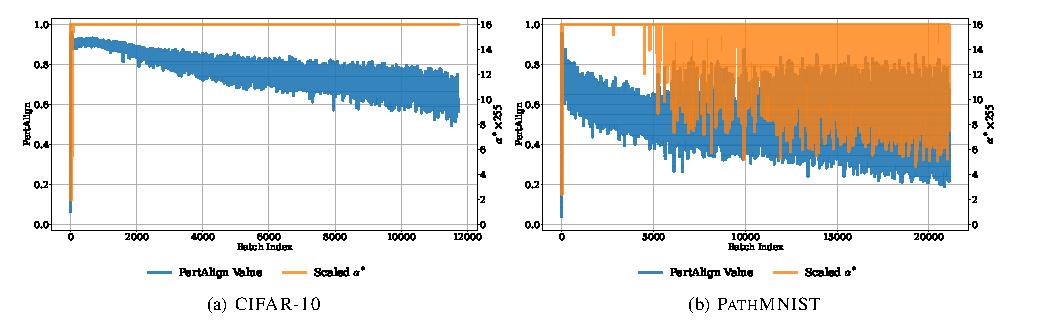
\includegraphics[width=\textwidth]{images/paper_stepsize.pdf}
\caption[تغییرات هم‌راستایی آشفتگی و سقف تطبیقی گام]{تغییرات \pertalign{} و سقف تطبیقی گام در آموزش گزارش‌شدهٔ مقاله برای \lr{CIFAR-10} و \lr{PATH MNIST}. ماندن روی سقف در بخش بزرگی از نمودار نخست و تنظیم‌های مکرر در نمودار دوم، رفتار متفاوت کنترل‌کننده را نشان می‌دهد. منحنی گام عملی، بهینهٔ دقیق هر نمونه در مدل درجه‌دو نیست. بازنشر از شکل ۵ مقالهٔ \sora{} \cite{sora2026}.}
\label{fig:method-stepsize}
\end{figure}

\section{مرز آموزش و مجموعهٔ تهدید ارزیابی}
\label{sec:method-budget}

طبق الگوریتم ۱ مقاله، نمونهٔ آموزشی از رابطهٔ
\begin{equation}
\widetilde x=\Pi_{[0,1]^d}\left(x+\eta+a\odot p\right)
\label{eq:method-training-clipping}
\end{equation}
ساخته می‌شود. در اینجا تصویرکردن فقط روی بازهٔ معتبر پیکسل‌هاست؛ تصویرکردن اضافی روی $x+[-\epsilon,\epsilon]^d$ وجود ندارد. نقطهٔ محاسبهٔ شیب نخست، $x+\eta$، نیز در شبه‌کد چاپ‌شده پیش از آن برش نمی‌خورد. افزودن چنین برشی یا محدود کردن آشفتگی کل به کرهٔ $\epsilon$، الگوریتم متفاوتی می‌سازد و باید به‌عنوان تغییر روش اعلام شود.

چون $|\eta_j|\leq\epsilon$، $0\leq a_j\leq\alpha_{\max}$ و $|p_j|\leq1$، برای آشفتگی خام داریم
\begin{equation}
\|\eta+a\odot p\|_\infty\leq\epsilon+\alpha_{\max}=3\epsilon
\label{eq:method-three-epsilon}
\end{equation}
که برابری آخر مربوط به انتخاب $\alpha_{\max}=2\epsilon$ است. برش بازهٔ پیکسل برای $x\in[0,1]^d$ فاصلهٔ مؤلفه‌ای از $x$ را افزایش نمی‌دهد، ولی آن را الزاماً تا $\epsilon$ کاهش نمی‌دهد. پس نمونه‌های آموزش ممکن است بیرون از کرهٔ $\epsilon$ باشند و عدد $3\epsilon$ یک کران بالا بر دامنهٔ ممکن است، نه اندازهٔ ثابت همهٔ نمونه‌ها.

در ارزیابی ستبری، مجموعهٔ تهدید همچنان اشتراک کرهٔ $\ell_\infty$ با شعاع $\epsilon$ و دامنهٔ معتبر تصویر است. حملهٔ ارزیابی باید این قید را رعایت کند و درستی گزارش‌شده به همان شعاع نسبت داده شود. استفاده از دامنهٔ بزرگ‌تر در آموزش، مجوز تغییر شعاع آزمون یا ادعای حل دقیق مسئلهٔ درونی با شعاع آموزشی نیست. این تفکیک برای مقایسه با آموزش‌های مبتنی بر \lr{PGD} و شروع تصادفی استاندارد ضروری است \cite{madry2018towards,wong2020fast,sora2026}.

\section{پیچیدگی، اجرای مشتق و حدود اعتبار}
\label{sec:method-complexity}

برای هر دسته، یک گذر برای محاسبهٔ شیب ورودی در نقطهٔ شروع و یک گذر روی نمونهٔ هم‌آورد برای مشتق پارامترها لازم است. مشتق ورودی انتهایی نیز همراه گذر دوم دریافت می‌شود. هزینهٔ نمونه‌برداری، ضرب مؤلفه‌ای و تجمیع نسبت‌ها برای $B$ نمونهٔ $d$بعدی از مرتبهٔ $O(Bd)$ است و حالت پایدار کنترل‌کننده تنها چند اسکالر دارد. نگهداری شیب‌ها و بردارهای حمله به حافظهٔ متناسب با ورودی نیاز دارد. در مقابل، ساخت صریح هسین حافظهٔ $O(d^2)$ و حل دستگاه مربوط به آن هزینهٔ اضافی چشمگیری می‌طلبد؛ هیچ‌یک جزء الگوریتم حاضر نیست.

ادعای اطلاعات مرتبهٔ دوم تقریباً رایگان، نسبت به گذرهای لازم در آموزش تک‌گامی بیان می‌شود. زمان و حافظه دقیقاً صفر نیستند و به چارچوب مشتق‌گیری و معماری بستگی دارند. مزیت اصلی، ثابت ماندن تعداد گذرهای شبکه و پرهیز از یک حلقهٔ چندگامی برای کاوش تازه است. در مقایسه با منظم‌سازی‌هایی که از خود معیار هم‌راستایی مشتق می‌گیرند، ذخیرهٔ گراف مشتقات مرتبهٔ بالاتر نیز لازم نیست \cite{andriushchenko2020understanding,sora2026}.

هنگام ساخت حمله، شیب و علامت آن باید از گراف به‌روزرسانی پارامترها جدا شوند. نمونهٔ نهایی سپس به‌عنوان ورودی مستقلی برای گذر دوم در نظر گرفته می‌شود تا هم مشتق آن ورودی و هم مشتق پارامترها قابل دریافت باشد. اگر هزینه در دسته میانگین گرفته می‌شود، مقیاس‌بندی دو شیب باید سازگار باشد؛ ضرب هر دو در یک ضریب مشترک، نسبت را تغییر نمی‌دهد، ولی ترکیب شیب مجموع و شیب میانگین نتیجه را عوض می‌کند. مشتق انتهایی باید نسبت به خود ورودی هم‌آورد باشد، نه صرفاً نسبت به ورودی پیش از عمل برش که ممکن است مؤلفه‌های مشتق را صفر کند.

محدودیت‌های اصلی از تقریب محلی و تفاوت آن با مسیر اجرایی می‌آیند. سطح واقعی در یک گام بلند لزوماً درجه‌دو نیست؛ نمونه‌برداری مؤلفه‌ای مسیر اسکالر را تغییر می‌دهد؛ برش پیکسل‌ها هندسهٔ جابه‌جایی را عوض می‌کند؛ و میانگین گذشته متعلق به نمونه‌ها و پارامترهای دیگری است. نزدیک بودن \pertalign{} به یک نیز طبق بخش~\ref{sec:geometry-limits} کوچک بودن هسین را ثابت نمی‌کند. در نتیجه، هیچ‌یک از این اجزا به‌تنهایی گواه ستبری یا تضمین بهینگی حمله نیست.

کارکرد روش را باید در کنار ارزیابی مستقل چندگامی، بررسی اندازهٔ واقعی آشفتگی و پایش روند آموزش سنجید. شکل‌های \ref{fig:method-recovery} و \ref{fig:method-stepsize} سازوکار و رفتار گزارش‌شدهٔ مقاله را پشتیبانی می‌کنند، اما تعمیم آن‌ها به هر دادگان، معماری یا برنامهٔ آموزش نیازمند شواهد است. نتیجهٔ نظری دقیق این فصل، حل محدود مدل درجه‌دو و رابطهٔ کاوش آن است؛ نتیجهٔ روشی، تبدیل این اطلاعات به یک کنترل‌کنندهٔ تصادفی، هموارشده و دارای تأخیر برای آموزش سریع است.
